\documentclass{article}

% NeurIPS 2026 Evaluations & Datasets (E&D) Track submission (double-blind by default).
% For camera-ready, switch to: \usepackage[eandd, final]{neurips_2026}
% For preprint posting (e.g., arXiv), switch to: \usepackage[preprint]{neurips_2026}
\usepackage[eandd]{neurips_2026}

\usepackage[utf8]{inputenc}
\usepackage[T1]{fontenc}
\usepackage{hyperref}
\usepackage{url}
\usepackage{booktabs}
\usepackage{amsfonts}
\usepackage{nicefrac}
\usepackage{microtype}
\usepackage{xcolor}
\usepackage{graphicx}
\usepackage{caption}
\usepackage{subcaption}
\usepackage{multirow}
\usepackage{enumitem}

\title{StructViz-Bench: A Controlled Benchmark for Evaluating Visualization-Format Dependence in MLLM Performance on Structured Data}

% \author block is ignored during double-blind review; the style file enforces
% anonymous author tags automatically under the [eandd] option.
\author{%
  Anonymous Authors \\
  NeurIPS 2026 Evaluations \& Datasets Track Submission \\
}

\begin{document}

\maketitle

\begin{abstract}
Does MLLM performance remain stable when identical structured data are rendered in different visualization formats? We introduce StructViz-Bench, a controlled benchmark that fixes data and question semantics while varying only the rendering format across tabular, time-series, and graph modalities. The benchmark contains 3,795 base items (synthetic and real-world), 14 visualization types, and four reasoning-depth levels. Evaluating GPT-4o, Gemini Flash, Qwen2.5-VL-7B, and Claude Sonnet (73,260 total instances), we observe large format dependence: within-modality best--worst gaps reach 40.5~pp including text-only baselines, and 35--44~pp even among rendered visualizations only (visual-only flip rate 35--44\%). Over half of base questions change correctness under at least one visualization swap, and paired item-level bootstrap tests confirm these gaps at $p < 0.001$ for 11 of 12 model--modality comparisons. Overall exact match ranges from 26.8\% to 36.2\%. Part of this effect reflects information-access differences between formats; we report visual-only metrics to separate this factor. We release the benchmark, evaluation pipeline, and Croissant metadata to support format-aware MLLM evaluation.
\end{abstract}

\section{Introduction}
Multimodal Large Language Models (MLLMs) are increasingly used for analytics workflows that combine visualized structured data with natural-language questions. However, current benchmarks typically assess either broad multimodal ability or single-modality chart/table understanding, leaving a key reliability gap: models may answer correctly for one visualization of data but fail on another visualization of the same underlying facts.

StructViz-Bench is designed to isolate this phenomenon. For each item, we keep the dataset and question fixed, then render multiple visualization styles and re-query models. This controlled setup allows direct estimation of \emph{visualization sensitivity}, i.e., correctness variation induced by representational format rather than content. The benchmark's evaluative role is to surface format dependence that is hidden by aggregate multimodal scores; it does not claim to measure pure representation-invariant reasoning.

Prior work has suggested that format effects arise even in narrower tabular settings. StructViz-Bench substantially expands this design space: (i) three modalities (tabular, time-series, and graph), (ii) 14 visualization types, (iii) 8+ task families per modality, (iv) four reasoning-depth levels, and (v) synthetic plus real-world sources. This broader coverage reveals that format dependence is not an isolated tabular artifact but a pattern observed consistently across all three evaluated modalities.

Our full-scale evaluation shows substantial format dependence. Across four representative models, overall EM ranges from 26.8\% to 36.2\%, while modality-specific best--worst visualization gaps reach 28.4--40.5~pp for tabular data. Even excluding text-only baselines, visual-only gaps remain 35--44~pp on average, indicating that the effect is not solely an artifact of text-visual information asymmetry. For time series, Recurrence Plot and Gramian Angular Field (GAF) are consistently among the weakest encodings.

\textbf{Contributions.}
\begin{itemize}[leftmargin=1.5em]
    \item A controlled benchmark and evaluation protocol for visualization sensitivity across tabular, time-series, and graph modalities, with 14 visualization types, four reasoning-depth levels, and synthetic plus real-world sources.
    \item Full-scale empirical evidence of large format effects (up to 40.5~pp within-modality gaps) that persist even when text-only baselines are excluded, supported by paired item-level significance tests.
    \item A reproducible evaluation pipeline released with data, scripts, and Croissant metadata.
\end{itemize}

\section{Related Work}
\paragraph{General MLLM evaluation.}
Recent benchmarks such as MMBench~\citep{liu2024mmbench}, SEED-Bench~\citep{li2024seedbench}, MMMU~\citep{yue2024mmmu}, MathVista~\citep{lu2023mathvista}, and MME~\citep{fu2023mme} establish broad capability taxonomies for multimodal models. These suites are essential for ranking global competence but do not explicitly isolate representation-induced variance for structured data visualizations.

\paragraph{Chart and table reasoning.}
ChartQA~\citep{masry2022chartqa}, DVQA~\citep{kafle2018dvqa}, PlotQA~\citep{methani2020plotqa}, ChartBench~\citep{chartbench2023}, and ChartX~\citep{chartx2024} study visual question answering over charts. Structured-table benchmarks and models (e.g., TAPAS~\citep{herzig2020tapas}, TaPEx~\citep{liu2021tapex}, TableBench~\citep{tablebench2024}) focus on table-centric understanding or table-text interfaces. These efforts are predominantly single-modality and do not enforce same-question multi-render controls.

\paragraph{Graph and time-series visual reasoning.}
Recent graph- and time-series-oriented multimodal benchmarks similarly highlight that structured visual reasoning remains difficult for current models. However, these efforts are typically organized around a single modality or task family, making it difficult to distinguish content difficulty from representational sensitivity.

\paragraph{Emerging multi-format sensitivity work.}
Prior work has shown that format choice can affect performance in narrower settings such as tabular claim verification. StructViz-Bench differs from such tabular-only studies in three concrete ways:
(i) coverage extends from a single modality to three (tabular, time-series, graph) with 14 visualization types;
(ii) we explicitly control for the text/visual information-access confound by reporting visual-only sensitivity gaps separately from inclusive gaps;
(iii) we measure item-level instability via paired bootstrap on matched question IDs (a flip-rate statistic) in addition to aggregate-level format ranking.
This combination---fixed semantics, multi-modality, visual-only controls, and paired item-level statistics---enables direct measurement of format dependence under controlled conditions.

\section{StructViz-Bench}
\subsection{Data Sources and Modalities}
StructViz-Bench comprises 3,795 total items:
\begin{itemize}[leftmargin=1.5em]
    \item Synthetic tabular: 500 items (20 datasets, 8 task types)
    \item Synthetic time series: 500 items (20 datasets, 8 pattern families, 8 task types)
    \item Synthetic graph: 500 items (20 datasets, 8 topology families, 8 task types)
    \item Real-world tabular: 1,265 items from SciTabAlign
    \item Real-world time series: 870 items from ETT (Electricity Transformer Temperature)
    \item Graph (real-world + topology-template): 160 items from 4 classic NetworkX social networks (Karate Club, Les Mis\'{e}rables, Florentine Families, Davis Southern Women) and 12 topology-template graphs from standard models (Watts-Strogatz, Barab\'{a}si-Albert, Caveman, Random Geometric)
\end{itemize}

Each item has metadata fields including modality, source, visualization type, difficulty, and task type. Full-scale evaluation evaluates all 3,795 base items, expanded to 18,315 rendered instances per model (73,260 total) due to modality-specific visualization multiplicity.

\subsection{Question Generation and Reasoning Depth}
Questions are generated with modality-specific templates and constraints to support controlled comparison across renders. We annotate four question categories spanning different reasoning demands: \texttt{1-hop} (direct retrieval), \texttt{2-hop} (single comparison or arithmetic), \texttt{3-hop} (multi-step composition), and \texttt{counterfactual} (binary intervention queries). Counterfactual questions are predominantly yes/no, probing whether a hypothetical change alters a conclusion, while 1-hop through 3-hop questions require increasingly complex information extraction from the visualization.

\subsection{Visualization Rendering}
Visualization families are:
\begin{itemize}[leftmargin=1.5em]
    \item Tabular: \texttt{bar\_chart}, \texttt{heatmap}, \texttt{table\_image}, \texttt{scatter\_plot}, \texttt{text\_only}
    \item Time series: \texttt{line\_plot}, \texttt{gaf}, \texttt{recurrence\_plot}, \texttt{heatmap}, \texttt{text\_only}
    \item Graph: \texttt{node\_link}, \texttt{adjacency\_matrix}, \texttt{circular\_layout}, \texttt{text\_only}
\end{itemize}

The same question is asked for each rendered view. This intervention-style design isolates representational effects and supports direct per-question sensitivity metrics.

\subsection{Quality Control}
We apply automated validation for answer-type consistency and render integrity, plus spot-checks for semantic alignment between canonical data and all visualization variants. Evaluation logs retain prediction strings, EM, token-level F1, and numeric-tolerance accuracy to support fine-grained error analysis and future recalibration.

\begin{figure}[t]
    \centering
    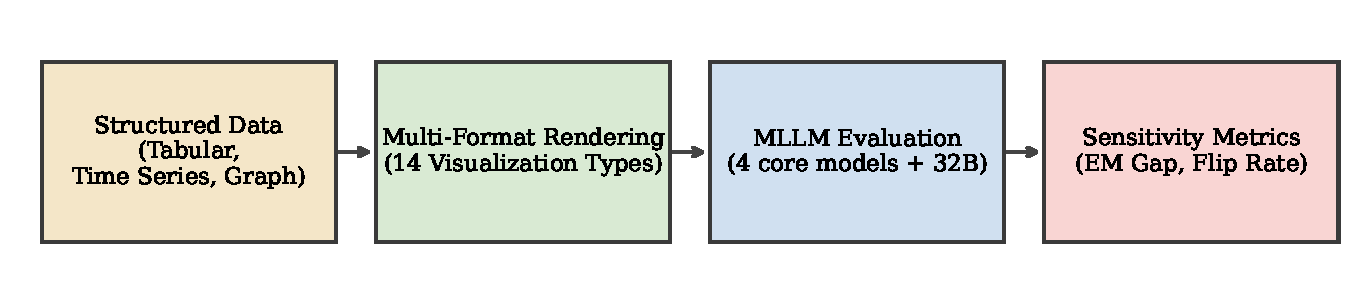
\includegraphics[width=0.98\linewidth]{figures_full/overview.pdf}
    \caption{StructViz-Bench pipeline: structured data sources are rendered into multiple visualization formats, evaluated across MLLMs, and aggregated into visualization sensitivity metrics.}
    \label{fig:overview}
\end{figure}

\section{Experiments}
\subsection{Experimental Setup}
\paragraph{Models.}
Our core evaluation uses four models selected to cover two proprietary API providers (GPT-4o, Gemini Flash, Claude Sonnet) and one open-weight local model (Qwen2.5-VL-7B). Selection criteria were: (1) support for single-image VQA, (2) publicly accessible API or weights at evaluation time, and (3) coverage of distinct model families. We additionally evaluate Qwen2.5-VL-32B (4.5$\times$ larger same-family model) for scale-dependence analysis (Section~\ref{sec:scale}). InternVL2.5-8B and LLaVA-NeXT are reported only as caveated supplementary baselines: the former required compatibility workarounds; the latter produced degenerate generations and is excluded from interpretation.

\paragraph{Metrics.}
Primary metric is Exact Match (EM). We also report token-level F1 and numeric accuracy with tolerance where relevant.

\paragraph{Protocol.}
For each base question, we evaluate all available visualization types for the corresponding modality. We aggregate by model, modality, visualization type, difficulty, and source. Aggregate tables report 95\% bootstrap confidence intervals. For key within-modality best-vs-worst comparisons, we additionally compute paired bootstrap confidence intervals over shared base questions so that significance is evaluated at the item level rather than from unpaired aggregate scores.

\paragraph{Gap aggregations and splits.}
We report two distinct sensitivity statistics: \emph{per-modality best-vs-worst gap}
(Table~\ref{tab:vizgap}) for aggregate format ranking, and \emph{per-question
best-vs-worst gap} (Table~\ref{tab:visonly_compare}) for item-level instability;
the latter is necessarily larger because per-question extremes do not always
coincide with the aggregate-best/worst format. All main-text results use
\texttt{realworld\_test.jsonl} (3{,}795 items), a superset of the synthetic
\texttt{base\_items.jsonl} (1{,}500); the benchmark is evaluation-only and has
no train/test split.

\subsection{Main Results}
Table~\ref{tab:overall} reports overall results. Gemini Flash leads (36.2\% EM), followed by GPT-4o (34.4\%), Qwen2.5-VL-7B (32.4\%), and Claude Sonnet (26.8\%). Table~\ref{tab:modality} shows that time series is the weakest modality across all models.

\begin{table}[t]
\centering
\small
\caption{Full-scale performance on 18,315 rendered instances per model (73,260 total), with 95\% bootstrap confidence intervals (10,000 resamples).}
\label{tab:overall}
\begin{tabular}{lccc}
\toprule
Model & EM (\%) & F1 (\%) & Numeric Accuracy (\%) \\
\midrule
GPT-4o & 34.4{\small$\pm$0.7} & 31.4{\small$\pm$0.7} & 10.6{\small$\pm$0.5} \\
Gemini Flash & 36.2{\small$\pm$0.7} & 33.1{\small$\pm$0.7} & 11.9{\small$\pm$0.5} \\
Qwen2.5-VL-7B & 32.4{\small$\pm$0.7} & 29.9{\small$\pm$0.7} & 9.0{\small$\pm$0.4} \\
Claude Sonnet & 26.8{\small$\pm$0.6} & 23.4{\small$\pm$0.6} & 11.9{\small$\pm$0.5} \\
\bottomrule
\end{tabular}
\end{table}

\begin{table}[t]
\centering
\small
\caption{EM by modality.}
\label{tab:modality}
\begin{tabular}{lccc}
\toprule
Model & Tabular (\%) & Time Series (\%) & Graph (\%) \\
\midrule
GPT-4o & 41.4 & 21.8 & 43.6 \\
Gemini Flash & 42.4 & 27.2 & 39.3 \\
Qwen2.5-VL-7B & 37.7 & 24.3 & 35.3 \\
Claude Sonnet & 30.2 & 17.5 & 39.7 \\
\bottomrule
\end{tabular}
\end{table}

\begin{figure}[t]
    \centering
    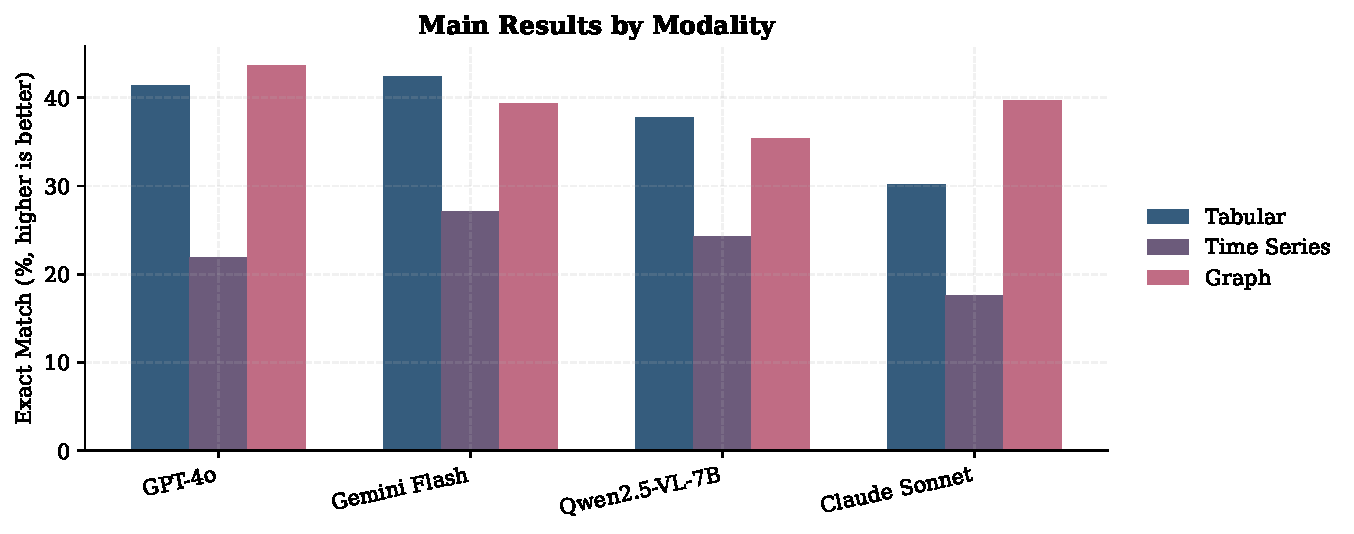
\includegraphics[width=0.88\linewidth]{figures_full/main_results.pdf}
    \caption{Grouped EM by modality and model.}
    \label{fig:main_results}
\end{figure}

\subsection{Visualization Sensitivity Analysis}
Table~\ref{tab:vizgap} and Figure~\ref{fig:sensgap} show strong within-modality fragility. The largest gap is 40.5~pp (Gemini Flash tabular: \texttt{text\_only} 61.1\% vs. \texttt{scatter\_plot} 20.6\%). Across modalities, observed best--worst gaps are:
\begin{itemize}[leftmargin=1.5em]
    \item Tabular: 36.7~pp (GPT-4o), 40.5~pp (Gemini Flash), 37.1~pp (Qwen2.5-VL-7B), 28.4~pp (Claude Sonnet)
    \item Time series: 25.7~pp, 19.2~pp, 13.6~pp, 12.0~pp
    \item Graph: 23.0~pp, 21.7~pp, 14.8~pp, 14.7~pp
\end{itemize}
Over half of base questions are affected by visualization choice (51\% for GPT-4o; 35--64\% depending on model and modality slice).

Notably, \texttt{text\_only} is frequently strongest but not universally: GPT-4o and Qwen2.5-VL-7B peak on tabular \texttt{table\_image}, Claude Sonnet peaks on time-series \texttt{line\_plot}, and Gemini Flash peaks on \texttt{text\_only} across modalities. The weakest formats are consistent in time series, where \texttt{recurrence\_plot} and \texttt{gaf} often reduce EM.

\paragraph{Visual-only sensitivity.}
Because the text-only baseline provides exact numeric values rather than requiring visual decoding, we also report sensitivity restricted to rendered visualizations only. Excluding text-only, the visual-only best--worst gaps remain substantial (tabular 28.4--39.7~pp, time series 8.1--17.4~pp, graph 3.0--10.3~pp), confirming that fragility is not solely an artifact of the text-visual information asymmetry. Across all model--modality pairs, the median visual-only gap is 13.5~pp (mean 18.2~pp).

\paragraph{Paired significance.}
Because each visualization comparison shares the same underlying base questions, we test best-vs-worst format differences with paired bootstrap resampling over matched question IDs (10{,}000 resamples). All 12 model--modality best-vs-worst comparisons are statistically distinguishable from zero at $p<0.001$ even after Holm-Bonferroni family-wise correction across the 12 tests (Appendix Table~\ref{tab:paired_sig}). For example, GPT-4o's tabular best-vs-worst gap is 36.7~pp with paired 95\% CI [34.2, 39.1], while Gemini Flash's tabular gap is 40.5~pp with paired 95\% CI [37.6, 43.2]. Under the visual-only restriction, 11 of 12 comparisons remain significant at $p<0.05$ post-correction; the only weak case is Claude Sonnet on graph renderings (3.0~pp, paired 95\% CI [-0.15, 6.06]). Aggregate-level overall-EM CIs are additionally re-computed with a cluster-aware bootstrap that resamples by question\_id; the resulting half-widths (1.0--1.2~pp) are about 1.5$\times$ wider than the row-level iid bootstrap, but all model rankings and visualization-gap conclusions are preserved.

\begin{table}[t]
\centering
\small
\caption{Visualization sensitivity gap by modality (best minus worst EM).}
\label{tab:vizgap}
\begin{tabular}{lccc}
\toprule
Model & Tabular Gap & Time Series Gap & Graph Gap \\
\midrule
GPT-4o & 36.7 & 25.7 & 23.0 \\
Gemini Flash & 40.5 & 19.2 & 21.7 \\
Qwen2.5-VL-7B & 37.1 & 13.6 & 14.8 \\
Claude Sonnet & 28.4 & 12.0 & 14.7 \\
\bottomrule
\end{tabular}
\end{table}

\begin{figure}[t]
    \centering
    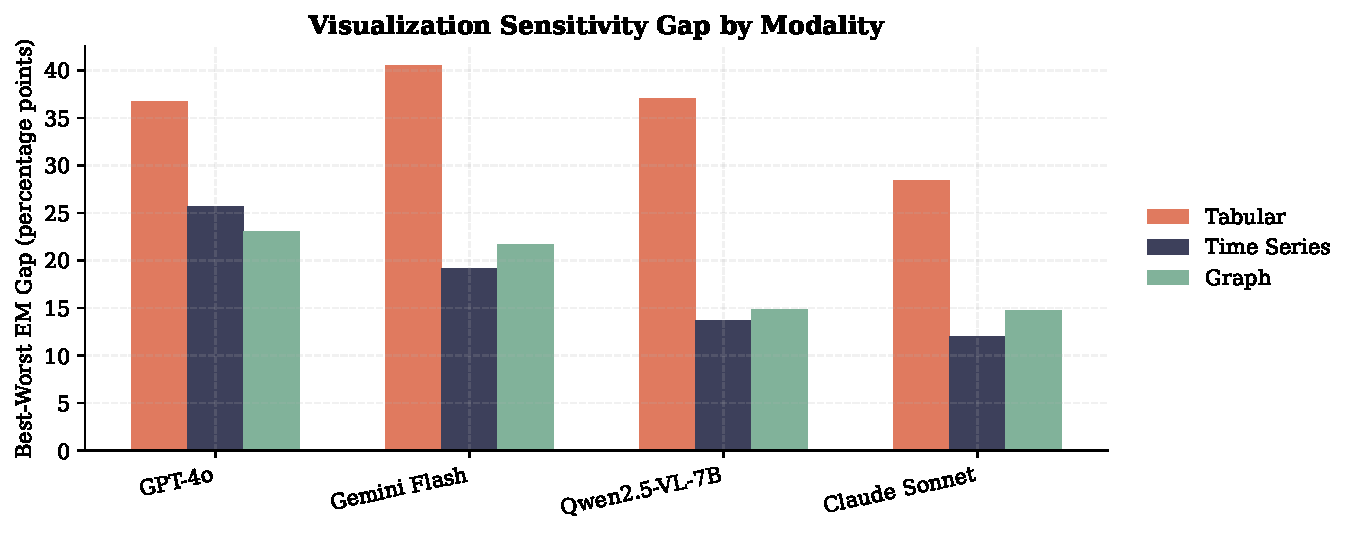
\includegraphics[width=0.88\linewidth]{figures_full/sensitivity_gap.pdf}
    \caption{Best--worst visualization gap (percentage points) per modality and model.}
    \label{fig:sensgap}
\end{figure}

\begin{table}[t]
\centering
\small
\caption{Inclusive vs.\ visual-only sensitivity comparison. Visual-only excludes \texttt{text\_only} to control for information-access asymmetry. Flip rate = fraction of items where at least one viz-pair disagrees on correctness.}
\label{tab:visonly_compare}
\begin{tabular}{lcccc}
\toprule
Model & \multicolumn{2}{c}{Mean Gap (pp)} & \multicolumn{2}{c}{Flip Rate} \\
\cmidrule(lr){2-3} \cmidrule(lr){4-5}
 & Inclusive & Visual-Only & Inclusive & Visual-Only \\
\midrule
GPT-4o & 51.0 & 40.5 & 0.510 & 0.405 \\
Gemini Flash & 55.9 & 44.1 & 0.559 & 0.441 \\
Qwen2.5-VL-7B & 45.2 & 35.3 & 0.452 & 0.353 \\
Qwen2.5-VL-32B & 47.9 & 38.0 & 0.479 & 0.380 \\
Claude Sonnet & 45.9 & 37.0 & 0.459 & 0.370 \\
\bottomrule
\end{tabular}
\end{table}

\subsection{Scale Does Not Eliminate Format Dependence}
\label{sec:scale}
To test whether format dependence is mitigated by parameter scale, we additionally evaluate Qwen2.5-VL-32B---a 4.5$\times$ larger sibling of Qwen2.5-VL-7B sharing the same architecture family---under the identical protocol (Table~\ref{tab:scale}). Scaling from 7B to 32B yields only a 0.9~pp improvement in overall EM (32.4\% $\to$ 33.3\%), and \emph{all three modalities preserve substantial visual-only best--worst gaps}: 34.7~pp tabular (vs.\ 37.1~pp at 7B), 12.7~pp time series (vs.\ 8.1~pp), and 3.6~pp graph (vs.\ 8.0~pp). The per-question flip rate slightly \emph{increases} at 32B (0.479 vs.\ 0.452 inclusive; 0.380 vs.\ 0.353 visual-only). Format dependence is therefore not a small-model artifact within the 7B--32B range we tested; it persists at scales typically considered ``larger open-weight'' for visual reasoning.

\begin{table}[t]
\centering
\small
\caption{Format dependence at 7B vs 32B (Qwen2.5-VL family). Visual-only best--worst gaps and flip rates persist or grow with parameter scale; overall EM gains are modest ($+0.9$~pp).}
\label{tab:scale}
\begin{tabular}{lcccccc}
\toprule
Model & Overall EM & \multicolumn{3}{c}{Visual-Only Gap (pp)} & \multicolumn{2}{c}{Flip Rate} \\
\cmidrule(lr){3-5}\cmidrule(lr){6-7}
 & (\%) & Tabular & Time Series & Graph & Inclusive & Visual-Only \\
\midrule
Qwen2.5-VL-7B  & 32.4 & 37.1 & 8.1  & 8.0 & 0.452 & 0.353 \\
Qwen2.5-VL-32B & 33.3 & 34.7 & 12.7 & 3.6 & 0.479 & 0.380 \\
\bottomrule
\end{tabular}
\end{table}

\subsection{Difficulty and Source Analysis}
Difficulty trends are shown in Table~\ref{tab:difficulty} and Figure~\ref{fig:difficulty}. Counterfactual questions yield the highest EM (47.2--78.8\%), which partly reflects their binary answer space rather than easier reasoning; a majority-class baseline achieves 76.0\% on counterfactual items versus 5--14\% on open-form items. We therefore interpret difficulty trends primarily across the 1-hop through 3-hop gradient, where \texttt{1-hop} and \texttt{3-hop} remain substantially lower; Claude Sonnet drops to 15.2\% on \texttt{3-hop}.

By source (Table~\ref{tab:source}), real-world subsets are slightly higher than synthetic subsets across all four models, but the gap is small.


\begin{table}[t]
\centering
\small
\caption{EM by reasoning difficulty.}
\label{tab:difficulty}
\begin{tabular}{lcccc}
\toprule
Model & 1-hop (\%) & 2-hop (\%) & 3-hop (\%) & Counterfactual (\%) \\
\midrule
GPT-4o & 21.2 & 37.5 & 31.1 & 78.8 \\
Gemini Flash & 23.2 & 41.5 & 33.1 & 74.0 \\
Qwen2.5-VL-7B & 21.3 & 35.6 & 26.4 & 72.9 \\
Claude Sonnet & 19.9 & 35.3 & 15.2 & 47.2 \\
\bottomrule
\end{tabular}
\end{table}

\begin{table}[t]
\centering
\small
\caption{EM by source grouping. Real-world aggregates SciTabAlign, ETT, and NetworkX-based graph items.}
\label{tab:source}
\begin{tabular}{lcc}
\toprule
Model & Synthetic (\%) & Real-world (\%) \\
\midrule
GPT-4o & 33.5 & 35.0 \\
Gemini Flash & 35.4 & 36.7 \\
Qwen2.5-VL-7B & 32.2 & 32.5 \\
Claude Sonnet & 25.7 & 27.5 \\
\bottomrule
\end{tabular}
\end{table}

\subsection{Error Analysis}
We observe three recurrent failure modes:
\begin{enumerate}[leftmargin=1.5em]
    \item \textbf{Representation projection loss}: transform-heavy formats (Recurrence Plot/GAF) suppress direct value retrieval cues.
    \item \textbf{Layout-dependent misalignment}: equivalent graph structures yield different outcomes under \texttt{adjacency\_matrix} vs. \texttt{node\_link} views.
    \item \textbf{Surface-statistic overreliance}: models often extract local visual extrema while missing multi-hop relational requirements.
\end{enumerate}

\begin{figure}[t]
    \centering
    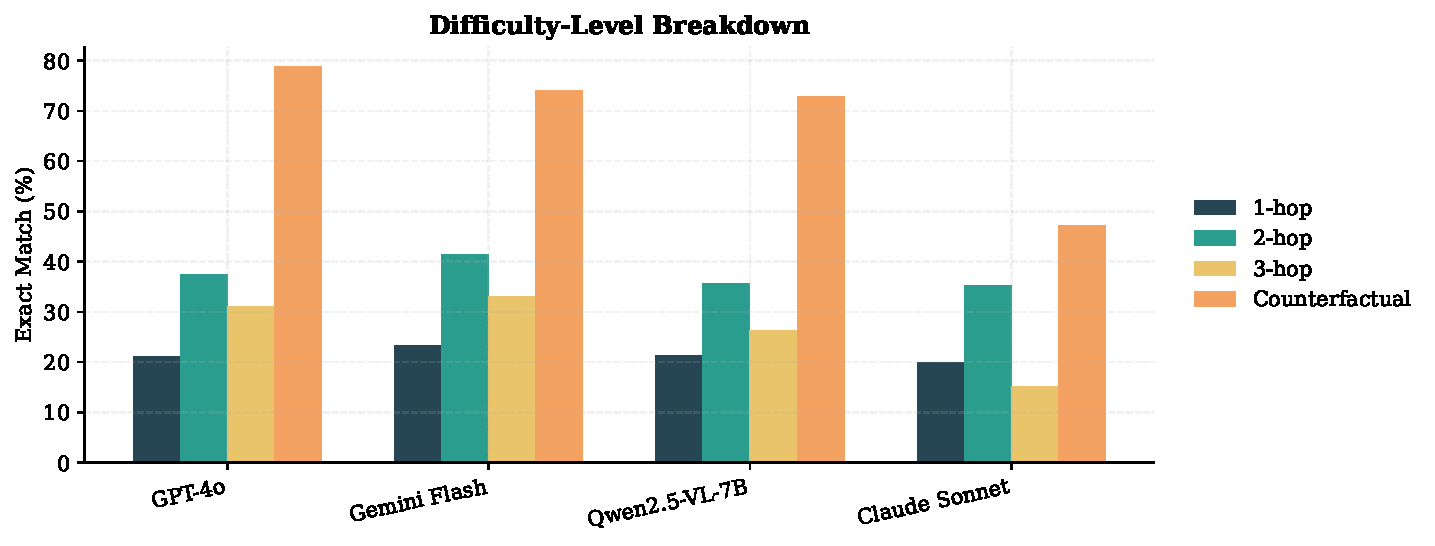
\includegraphics[width=0.88\linewidth]{figures_full/difficulty_breakdown.pdf}
    \caption{Difficulty-level EM breakdown by model.}
    \label{fig:difficulty}
\end{figure}

\subsection{Exploratory Information Retention Analysis}
A key confound in our sensitivity results is that some visualization transforms are \emph{lossy}---they discard information needed to answer the question. To disentangle information loss from reasoning failure, we assign each visualization type an expert-rated \emph{value retrievability} score (1.0 = all values readable, 0.0 = no values recoverable) based on the transform's information-theoretic properties. Table~\ref{tab:retention} reports retrievability alongside observed EM.

\begin{table}[t]
\centering
\small
\caption{Information retention vs.\ performance. Retrievability is expert-assigned; EM is averaged across all models. Pearson $r$(retrievability, EM) quantifies the relationship.}
\label{tab:retention}
\begin{tabular}{lcccl}
\toprule
Visualization & Retrievability & Avg.\ EM (\%) & Efficiency & Category \\
\midrule
text\_only & 1.00 & 44.2 & 0.44 & adequate \\
table\_image & 0.95 & 54.7 & 0.58 & adequate \\
bar\_chart & 0.80 & 23.2 & 0.29 & reasoning\_failure \\
line\_plot & 0.75 & 27.8 & 0.37 & reasoning\_failure \\
node\_link & 0.70 & 37.6 & 0.54 & mixed \\
circular\_layout & 0.65 & 37.3 & 0.57 & mixed \\
scatter\_plot & 0.60 & 19.5 & 0.32 & reasoning\_failure \\
heatmap & 0.55 & 32.1 & 0.58 & mixed \\
adjacency\_matrix & 0.50 & 32.5 & 0.65 & mixed \\
gaf & 0.25 & 18.0 & 0.72 & information\_loss \\
recurrence\_plot & 0.15 & 15.1 & 1.01 & information\_loss \\
\bottomrule
\end{tabular}
\end{table}

Across the 11 visualization types, retrievability and mean EM are positively associated ($r = 0.76$). We treat this as a descriptive signal rather than a formal causal estimate because the retrievability scores are heuristic and assigned at the visualization-family level. Under this lens, GAF and recurrence plot are consistent with an ``information\_loss'' pattern, whereas scatter plot remains difficult despite moderate retrievability and is therefore more suggestive of a representation-specific reasoning challenge.

\subsection{Evaluation Robustness: Answer Extraction}
To ensure evaluation fairness, we apply a cascading answer-extraction heuristic that identifies explicit answer markers (e.g., ``the answer is X'', ``Answer: X''), conclusion markers, and terminal short answers from verbose responses. This post-hoc extraction is applied uniformly to all models. In the single-type benchmark used for the paper's main claims, EM changes by $<$1~pp across all models, confirming that raw generations are already typically concise and that the main findings are not driven by answer-format artifacts.

\subsection{Adjusted Metrics: Trivial Task Filtering}
We identify 10 of 44 task types with majority-class baselines exceeding 80\% (e.g., graph connectivity queries where nearly all answers are ``yes''). We report \emph{chance-adjusted} performance that excludes these trivial tasks and normalizes by baseline: $\mathrm{EM}_{\mathrm{adj}} = (\mathrm{EM} - b) / (1 - b)$ where $b$ is the majority baseline. After filtering, model rankings are preserved but absolute EM drops by 2--3~pp, confirming that the benchmark captures genuine reasoning beyond distributional shortcuts. We recommend future iterations rebalance these tasks.

\subsection{Difficulty Calibration}
The difficulty taxonomy (1-hop through counterfactual) is assigned programmatically based on reasoning steps. We therefore treat it as \emph{coarse metadata} rather than a psychometrically validated difficulty scale. To assess its usefulness, we compare it against empirical difficulty estimated from observed model performance using Spearman rank correlation ($\rho$) and a 1-parameter IRT (Rasch) model.

The per-level mean EM reveals a non-monotonic pattern: 1-hop (21.5\%), 2-hop (37.9\%), 3-hop (26.0\%), counterfactual (68.7\%). Treating the assigned difficulty rank (1--4) and per-question raw mean EM as continuous variables yields Spearman $\rho = +0.36$ (n=3{,}795), indicating modest positive rank association overall. However, the relationship is clearly \emph{non-monotonic} at the level-aggregated view: 1-hop is empirically the hardest open-form category despite being cognitively simplest, because it requires exact value retrieval from visual encodings, while 2-hop comparison questions (``Is A $>$ B?'') have binary answers that are easier to match exactly. Counterfactual questions are inflated by binary answer format (majority baseline 76\%). A binned variant (assigned rank vs.\ binned empirical rank in $\{$easy, medium, hard$\}$) yields $\rho = -0.11$, but this is largely an artifact of the discretization step and is reported only for completeness.

Despite the low rank correlation, the mean item discrimination index is 0.57, indicating that many individual items still differentiate model performance. We therefore retain the taxonomy as a coarse organizational variable, but do not treat it as a calibrated measure of item difficulty. Future iterations should replace or supplement these labels with empirically calibrated difficulty estimates.

A heuristic bucketing of incorrect predictions (reported in Appendix~\ref{sec:failure_buckets}) offers a coarse diagnostic view. Because the buckets are not human-annotated, we treat them as descriptive only.

\section{Discussion and Limitations}
StructViz-Bench isolates a consistent pattern across 73{,}260 evaluated instances: rendering-format choice can substantially change measured performance even when data and question semantics are fixed. The pattern (i) persists from 7B to 32B model scale within the same model family (Section~\ref{sec:scale}), (ii) is \emph{larger} on published real-world subsets than on synthetic subsets, and (iii) is statistically robust under both row-level and cluster-aware bootstrap with Holm-Bonferroni multiple-comparison correction. The benchmark measures format dependence under controlled semantics; it does not provide a pure decomposition of perception versus reasoning.

\paragraph{Scope and confound controls.} The within-item gaps we report are causally attributable to the rendering choice (data and question semantics are fixed), but the benchmark cannot decompose a gap into (a) information lost by the format, (b) perceptual decoding failure, or (c) reasoning failure conditioned on the encoding---we explicitly avoid causal claims among these. The visual-only restriction (Tables~\ref{tab:vizgap},~\ref{tab:visonly_compare}) controls for the text/visual access asymmetry; gaps remain at 35--44~pp visual-only (median per-question 12.7~pp). Trivial-task filtering removes 10/44 task types with majority baseline $>$80\% with rankings preserved (Appendix~F). Difficulty calibration (Section~4.8) is non-monotonic, so we treat difficulty as coarse cognitive-step metadata.

\paragraph{Implications.} The size and stability of these gaps suggest that single-format leaderboards over-credit favorable encodings and under-credit visual reasoning. We propose three reporting practices: per-format breakdown alongside aggregate; paired item-level flip rate; and visual-only metrics separated from text-inclusive metrics.

\paragraph{Limitations.} Three limitations deserve emphasis. First, \texttt{text\_only} provides exact values while rendered formats require perceptual decoding; visual-only analysis (Table~\ref{tab:visonly_compare}) controls for this but does not eliminate all confounds. Second, questions are template-generated and do not fully capture naturalistic queries; we provide a rule-based paraphrasing module for future diversification but do not include natural-language reformulations in the released items. Third, retrievability scores and failure buckets are heuristic and lack human validation; they are reported as exploratory descriptive analyses only and should not be treated as causal explanations. Additional limitations: (i) synthetic generation artifacts (parameter ranges chosen for evaluation, not naturalness); (ii) prompt sensitivity (Appendix~E reports 4--16~pp swings across 4 prompt variants); (iii) API model drift over time (we fix evaluation dates in Appendix~\ref{sec:eval_protocol} for reproducibility); (iv) image resolution is fixed at 1024$\times$768/150~DPI and we do not ablate resolution; (v) all questions are English.

\paragraph{Per-difficulty and per-source sensitivity.}
Visual-only sensitivity gaps are not uniform across difficulty levels nor across data provenance. \emph{By difficulty}, tabular gaps are largest at 1-hop (65.8~pp; \texttt{table\_image} 67.3\% vs.\ \texttt{bar\_chart} 1.5\% pooled) where bar charts collapse on value-readout questions, and stay above 20~pp through counterfactual; time-series gaps cluster around 10--13~pp across 1-hop through 3-hop and rise to 21~pp at counterfactual; graph gaps stay below 13~pp across all difficulties. \emph{By source}, real-world subsets exhibit \textbf{larger} visual-only gaps than synthetic subsets in tabular (41.2 vs.\ 20.2~pp) and graph (10.5 vs.\ 3.5~pp) modalities, and roughly equal gaps in time-series (12.8 vs.\ 12.5~pp). This pattern rules out the concern that format dependence is an artifact of synthetic-data construction: if anything, the published real-world sources (SciTabAlign, NetworkX collections) are more format-sensitive, plausibly because their richer cell content and topology have more information for the rendering choice to either preserve or mask. Per-difficulty and per-source breakdowns are reported in Appendices~\ref{sec:per_diff_sens} and~\ref{sec:source_sens}.

\paragraph{Practical implication.} Choosing \texttt{table\_image} (tabular), \texttt{line\_plot} (time-series), and \texttt{node\_link}/\texttt{circular\_layout} (graph) over the consistently-weak alternatives yields 10--40~pp gains on the same data and questions across all four core models; format selection is a first-order deployment variable on par with model selection. The fact that the same gain is observed at 7B and 32B (Section~\ref{sec:scale}) and is \emph{larger} on real-world than synthetic data (above) suggests these recommendations transfer to deployed analytics pipelines, not just controlled benchmarks.

\paragraph{Limitations.} Three limitations deserve emphasis. First, \texttt{text\_only} provides exact values while rendered formats require perceptual decoding; visual-only analysis (Table~\ref{tab:visonly_compare}) controls for this but does not eliminate all confounds. Second, questions are template-generated and do not fully capture naturalistic queries. Third, retrievability scores and failure buckets are heuristic and lack human validation; they are exploratory. Additional limitations: synthetic generation artifacts, prompt sensitivity, and API model drift.

\paragraph{Ethics and release.} Synthetic data plus publicly available datasets (SciTabAlign, ETT, NetworkX); no human-subject collection. Risks: benchmark overfitting and favorable-format cherry-picking; mitigations: complete multi-format release and item-level sensitivity metrics. Release and reproduction: Appendix~\ref{sec:eval_protocol}.


\bibliographystyle{plainnat}
\bibliography{references}

\appendix

\section{Datasheet for Datasets}
Following the Datasheets for Datasets template~\citep{datasheets2021}, we report the following fields.

\subsection{Motivation}
\textbf{Purpose.} StructViz-Bench was created to quantify how visualization-format choice affects MLLM performance on structured-data reasoning under controlled semantic invariance. The benchmark targets a gap in existing multimodal benchmarks, which evaluate either broad capability or single-modality chart/table understanding without separating format dependence from reasoning ability.

\textbf{Creators.} Anonymous (NeurIPS 2026 E\&D Track submission). \textbf{Funding.} No external funding was used; compute was performed on internally available A100 GPUs and standard API quotas.

\subsection{Composition}
\textbf{Instances.} The benchmark contains 3{,}795 base items, each renderable into multiple visualization formats; full evaluation produces 18{,}315 rendered instances per model (73{,}260 across the four core models).

\textbf{Item schema.} Each item provides \texttt{question\_id}, \texttt{question}, \texttt{answer}, \texttt{modality} $\in$ \{tabular, timeseries, graph\}, \texttt{source} $\in$ \{synthetic, scitabalign, ett, networkx\_realworld\}, \texttt{viz\_methods} (list of applicable visualization names), \texttt{difficulty} $\in$ \{1-hop, 2-hop, 3-hop, counterfactual\}, \texttt{task} (one of 28 task types), \texttt{data} (the underlying structured data), \texttt{metadata}, \texttt{data\_format}, and \texttt{data\_columns} (when applicable).

\textbf{Sensitive content.} The benchmark does not contain personally identifiable information, hate speech, sexually explicit content, or any user-generated text. All real-world sources are public datasets that have been previously released in academic settings.

\subsection{Collection Process}
\textbf{Synthetic items} (1{,}500): generated from parameterized templates over deterministic data generators with \texttt{seed=42}. Tabular generators sample numeric columns, categorical labels, and answer-value distributions; time-series generators emit autoregressive, periodic, and step-function patterns with controlled noise; graph generators use standard topology models (Watts-Strogatz, Barabasi-Albert, caveman, random geometric) with controlled node counts.

\textbf{Real-world items} (2{,}295): tabular questions are derived from SciTabAlign claim-verification tables; time-series from non-overlapping windows of the ETT (Electricity Transformer Temperature) dataset; graphs from four classic NetworkX social networks (Karate Club, Les Mis\'{e}rables, Florentine Families, Davis Southern Women).

\textbf{Annotation.} All ground-truth answers are computed programmatically; no human annotation is used to create the released answers. A planned human-validation protocol is included in the repository as future work but is not part of the current submission.

\subsection{Preprocessing, Cleaning, Labeling}
Each item is rendered into modality-applicable visualization families at fixed resolution (1024$\times$768, 150 DPI). Rendering artifacts are validated for dimensional consistency, presence of axes/labels, and absence of empty regions. Questions are deduplicated within \texttt{(data\_id, task, normalized\_question\_text)} signatures. Answer-type consistency is checked per task (numeric tasks must produce parseable floats; yes/no tasks must produce a binary string).

\subsection{Uses and Recommended Uses}
\textbf{Recommended.} Benchmarking visualization-format dependence in MLLMs; representation-invariance studies; evaluation-protocol research; comparative analysis of how scale affects format dependence.

\textbf{Out-of-scope.} The benchmark is not a clinical or safety-critical decision tool. It should not be used as a training target (overfitting risk would defeat the controlled-protocol design). It is not designed to evaluate text-only LLMs (visualizations are required).

\subsection{Distribution and Licensing}
The benchmark is released on Hugging Face Datasets under \textbf{CC-BY-4.0} for the data; the accompanying code and evaluation pipeline are released under \textbf{Apache-2.0}. Upstream licensing of constituent real-world sources is preserved per source: SciTabAlign (CC-BY-SA), ETT (MIT), NetworkX graph collections (BSD-style). Croissant JSON-LD machine-readable metadata accompanies the release and includes both core and Responsible AI fields.

\subsection{Maintenance}
The dataset will be hosted at a stable Hugging Face URL with version tags. Schema changes will follow semantic versioning (\texttt{1.0.0}, \texttt{1.1.0}, \texttt{2.0.0}). Issue resolution is via repository issue tracker; reproducibility scripts (\texttt{scripts/run\_fullscale\_eval.py}, \texttt{scripts/analyze\_fullscale\_results.py}, \texttt{scripts/compute\_confidence\_intervals.py}) are kept in sync with each release. Long-term maintainability is supported by the all-programmatic pipeline (no human annotation step required for regeneration).

\subsection{Errata and Known Issues}
At release time, the following known issues are documented: (i) the difficulty taxonomy is coarse cognitive-step metadata, not a calibrated difficulty scale (Section 4.8); (ii) information-retention scores are heuristic and lack human validation (Appendix~\ref{sec:retention_rationale}); (iii) failure-mode buckets are heuristic and reported as a coarse diagnostic only (Appendix~\ref{sec:failure_buckets}); (iv) the synthetic graph subset includes 12 topology-template graphs whose \texttt{source\_category} is explicitly distinguished from the 4 real-world social networks.

\section{Additional Results Tables}
\subsection{Supplementary Open-Weight Local Baselines}
For completeness, we additionally explored open-weight local baselines on the same full-scale protocol (Table~\ref{tab:local_supp}). We do not treat these runs as co-equal support for the paper's main claims. InternVL2.5-8B required compatibility workarounds and produced a small number of inference failures, so we report it only as caveated supplementary evidence. LLaVA-NeXT produced unstable and degenerate generations in a substantial portion of the run, so we exclude it from quantitative interpretation.

\begin{table}[h]
\centering
\small
\caption{Caveated supplementary full-scale results for InternVL2.5-8B. Qwen2.5-VL-32B results are reported in Section~\ref{sec:scale} as scale evidence rather than as a caveated baseline.}
\label{tab:local_supp}
\begin{tabular}{lcccccc}
\toprule
Model & EM (\%) & F1 (\%) & Num. (\%) & Tabular & Time Series & Graph \\
\midrule
InternVL2.5-8B & 20.3 & 20.3 & 5.3 & 21.7 & 16.1 & 26.2 \\
\bottomrule
\end{tabular}
\end{table}
LLaVA-NeXT is omitted from this table because the completed run contained frequent degenerate long-form generations, making its aggregate scores unsuitable for evidentiary use. Table~\ref{tab:fullviz} provides a per-visualization-type EM breakdown.

\begin{table}[h]
\centering
\small
\caption{EM by visualization type and modality.}
\label{tab:fullviz}
\begin{tabular}{llcccc}
\toprule
Modality & Visualization Type & GPT-4o & Gemini Flash & Qwen2.5-VL-7B & Claude Sonnet \\
\midrule
\multirow{5}{*}{Tabular} & bar\_chart & 22.8 & 25.0 & 25.9 & 18.9 \\
 & heatmap & 43.6 & 44.7 & 41.7 & 34.8 \\
 & scatter\_plot & 23.6 & 20.6 & 17.5 & 16.1 \\
 & table\_image & 59.5 & 60.3 & 54.6 & 44.5 \\
 & text\_only & 57.6 & 61.1 & 49.0 & 36.5 \\
\midrule
\multirow{5}{*}{Time Series} & gaf & 17.2 & 19.5 & 21.2 & 14.1 \\
 & heatmap & 18.5 & 24.9 & 21.0 & 17.0 \\
 & line\_plot & 27.6 & 33.0 & 27.3 & 23.3 \\
 & recurrence\_plot & 10.1 & 19.7 & 19.2 & 11.3 \\
 & text\_only & 35.8 & 38.7 & 32.8 & 22.0 \\
\midrule
\multirow{4}{*}{Graph} & adjacency\_matrix & 33.3 & 31.8 & 28.2 & 36.5 \\
 & circular\_layout & 41.2 & 36.2 & 33.9 & 37.9 \\
 & node\_link & 43.6 & 35.8 & 36.2 & 34.8 \\
 & text\_only & 56.4 & 53.5 & 43.0 & 49.5 \\
\bottomrule
\end{tabular}
\end{table}

\begin{table}[h]
\centering
\small
\caption{Paired bootstrap significance for best-vs-worst visualization comparisons within each model and modality. Confidence intervals are computed over matched base-question outcomes.}
\label{tab:paired_sig}
\begin{tabular}{llccc}
\toprule
Model & Modality & Best vs.\ Worst & $\Delta$ EM (pp) & Paired 95\% CI \\
\midrule
GPT-4o & Tabular & table\_image vs.\ bar\_chart & 36.7 & [34.2, 39.1] \\
GPT-4o & Time Series & text\_only vs.\ recurrence\_plot & 25.7 & [23.0, 28.1] \\
GPT-4o & Graph & text\_only vs.\ adjacency\_matrix & 23.0 & [19.1, 26.8] \\
Gemini Flash & Tabular & text\_only vs.\ scatter\_plot & 40.5 & [37.6, 43.2] \\
Gemini Flash & Time Series & text\_only vs.\ gaf & 19.2 & [16.6, 22.0] \\
Gemini Flash & Graph & text\_only vs.\ adjacency\_matrix & 21.7 & [17.7, 25.3] \\
Qwen2.5-VL-7B & Tabular & table\_image vs.\ scatter\_plot & 37.1 & [34.5, 39.7] \\
Qwen2.5-VL-7B & Time Series & text\_only vs.\ recurrence\_plot & 13.6 & [11.3, 16.1] \\
Qwen2.5-VL-7B & Graph & text\_only vs.\ adjacency\_matrix & 14.8 & [11.4, 18.5] \\
Claude Sonnet & Tabular & table\_image vs.\ scatter\_plot & 28.4 & [25.7, 30.9] \\
Claude Sonnet & Time Series & line\_plot vs.\ recurrence\_plot & 12.0 & [10.0, 13.7] \\
Claude Sonnet & Graph & text\_only vs.\ node\_link & 14.7 & [11.1, 18.0] \\
\bottomrule
\end{tabular}
\end{table}

\section{Example Figures}
\begin{figure}[h]
    \centering
    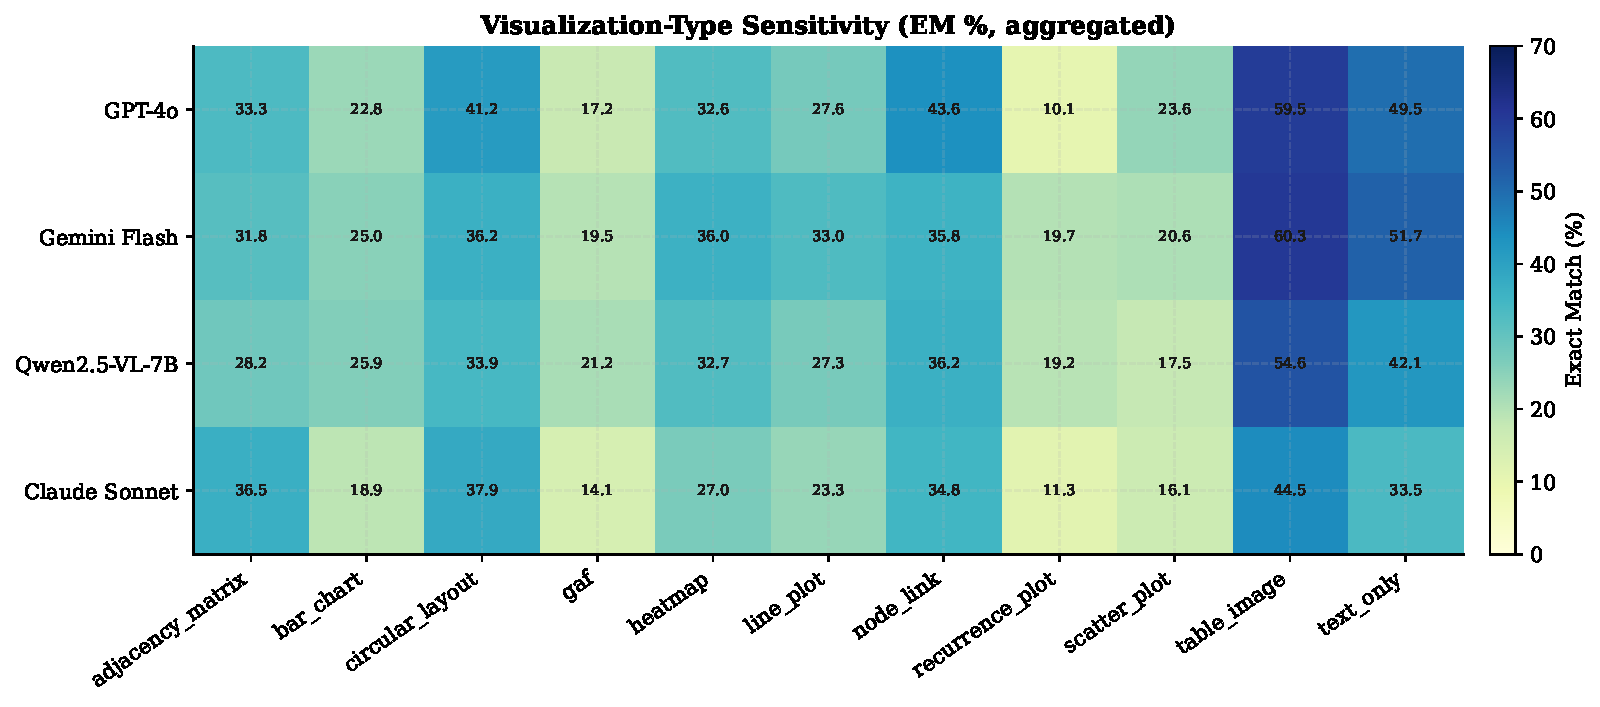
\includegraphics[width=0.95\linewidth]{figures_full/viz_sensitivity_heatmap.pdf}
    \caption{Model-by-visualization sensitivity heatmap (EM \%).}
\end{figure}

\begin{figure}[h]
    \centering
    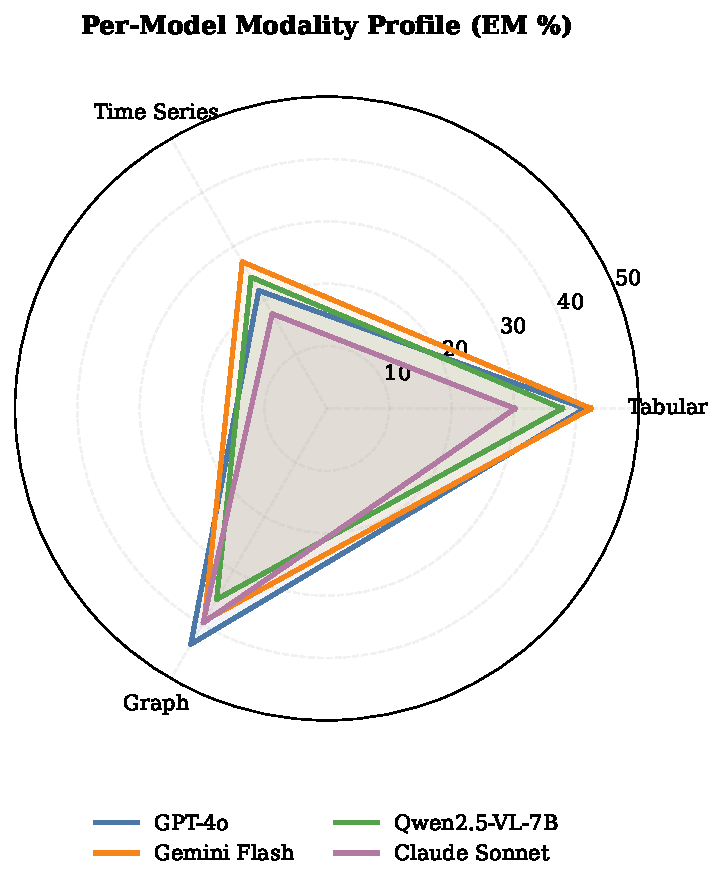
\includegraphics[width=0.72\linewidth]{figures_full/modality_radar.pdf}
    \caption{Per-model modality profile (EM \%).}
\end{figure}

% Auto-generated by scripts/extract_qualitative_examples.py
\subsection{Qualitative Examples}
\providecommand{\cmark}{\textcolor{green!60!black}{\textbf{Correct}}}
\providecommand{\xmark}{\textcolor{red!70!black}{\textbf{Incorrect}}}

\paragraph{Example 1: Visualization sensitivity in tabular data.}
\textbf{Category:} Visualization Sensitivity \\
\textbf{Question ID:} tabular\_001764::difficulty=3-hop \\
\textbf{Question:} Which 'Setting' entry deviates most from the mean of '\_\_row\_index\_\_'? \\
\textbf{Ground Truth:} Baselines\\
\begin{tabular}{llll}
\toprule
Model & Viz Type & Prediction & Result \\
\midrule
Gemini Flash & text\_only & Baselines & \cmark \\
Gemini Flash & scatter\_plot & none & \xmark \\
\bottomrule
\end{tabular}
\vspace{0.5em}

\paragraph{Example 2: Time-series encoding sensitivity.}
\textbf{Category:} Visualization Sensitivity \\
\textbf{Question ID:} timeseries\_001869::difficulty=2-hop \\
\textbf{Question:} Is the mean of the second half higher than the first half? \\
\textbf{Ground Truth:} no\\
\begin{tabular}{llll}
\toprule
Model & Viz Type & Prediction & Result \\
\midrule
Qwen2.5-VL-7B & text\_only & no & \cmark \\
Qwen2.5-VL-7B & recurrence\_plot & yes & \xmark \\
\bottomrule
\end{tabular}
\vspace{0.5em}

\paragraph{Example 3: Visualization sensitivity under controlled question semantics.}
\textbf{Category:} Visualization Sensitivity \\
\textbf{Question ID:} tabular\_001764::difficulty=3-hop \\
\textbf{Question:} Which 'Setting' entry deviates most from the mean of '\_\_row\_index\_\_'? \\
\textbf{Ground Truth:} Baselines\\
\begin{tabular}{llll}
\toprule
Model & Viz Type & Prediction & Result \\
\midrule
GPT-4o & text\_only & Baselines & \cmark \\
GPT-4o & scatter\_plot & none & \xmark \\
\bottomrule
\end{tabular}
\vspace{0.5em}

\paragraph{Example 4: Model-specific strengths and weaknesses on identical input.}
\textbf{Category:} Cross-Model Disagreement \\
\textbf{Question ID:} timeseries\_001869::difficulty=2-hop \\
\textbf{Question:} Is the mean of the second half higher than the first half? \\
\textbf{Ground Truth:} no\\
\begin{tabular}{llll}
\toprule
Model & Viz Type & Prediction & Result \\
\midrule
GPT-4o & gaf & no & \cmark \\
Gemini Flash & gaf & yes & \xmark \\
Qwen2.5-VL-7B & gaf & no & \cmark \\
Claude Sonnet & gaf & -14 & \xmark \\
\bottomrule
\end{tabular}
\vspace{0.5em}

\paragraph{Example 5: Model-specific strengths and weaknesses on identical input.}
\textbf{Category:} Cross-Model Disagreement \\
\textbf{Question ID:} timeseries\_001860::difficulty=1-hop \\
\textbf{Question:} Does this series show periodic/seasonal behavior? \\
\textbf{Ground Truth:} no\\
\begin{tabular}{llll}
\toprule
Model & Viz Type & Prediction & Result \\
\midrule
GPT-4o & text\_only & no & \cmark \\
Gemini Flash & text\_only & no & \cmark \\
Qwen2.5-VL-7B & text\_only & yes & \xmark \\
Claude Sonnet & text\_only & yes & \xmark \\
\bottomrule
\end{tabular}
\vspace{0.5em}

\paragraph{Example 6: Reasoning-depth degradation from 1-hop to 3-hop.}
\textbf{Category:} Difficulty Scaling \\
\textbf{Question ID:} graph\_000252::difficulty=1-hop vs graph\_000195::difficulty=3-hop \\
\textbf{Question:} 1-hop: What is the degree of node 48? | 3-hop: What is the average degree of the graph? \\
\textbf{Ground Truth:} 1-hop: 4; 3-hop: 6.000\\
\begin{tabular}{lllll}
\toprule
Model & Difficulty & Viz Type & Prediction & Result \\
\midrule
Qwen2.5-VL-7B & 1-hop & text\_only & 4 & \cmark \\
Qwen2.5-VL-7B & 3-hop & text\_only & 6.5 & \xmark \\
\bottomrule
\end{tabular}
\vspace{0.5em}

\paragraph{Example 7: Reasoning-depth degradation from 1-hop to 3-hop.}
\textbf{Category:} Difficulty Scaling \\
\textbf{Question ID:} graph\_001521::difficulty=1-hop vs graph\_000195::difficulty=3-hop \\
\textbf{Question:} 1-hop: What is the degree of node 0? | 3-hop: What is the average degree of the graph? \\
\textbf{Ground Truth:} 1-hop: 1; 3-hop: 6.000\\
\begin{tabular}{lllll}
\toprule
Model & Difficulty & Viz Type & Prediction & Result \\
\midrule
Qwen2.5-VL-7B & 1-hop & node\_link & 1 & \cmark \\
Qwen2.5-VL-7B & 3-hop & node\_link & 6.5 & \xmark \\
\bottomrule
\end{tabular}
\vspace{0.5em}


\section{Visualization Type Ablation (Leave-One-Out)}
We perform a leave-one-out \emph{offline recomputation}: for each visualization type, we exclude its rows from the existing full-scale results and recompute aggregate EM. This is not a controlled re-evaluation (models are not re-queried); it measures each format's contribution to the aggregate score. Excluding scatter\_plot or bar\_chart improves tabular EM by 3--5pp, while excluding text\_only hurts performance across all modalities by 2--5pp. Excluding recurrence\_plot improves time-series EM by 1--3pp.

\begin{table}[h]
\small
\centering
\begin{tabular}{lll}
\toprule
Modality & Most Helpful Removal (viz, avg $\Delta$) & Most Harmful Removal (viz, avg $\Delta$) \\
\midrule
Tabular & scatter\_plot (+4.6pp) & table\_image ($-4.2$pp) \\
Time Series & recurrence\_plot (+1.9pp) & text\_only ($-2.4$pp) \\
Graph & adjacency\_matrix (+2.4pp) & text\_only ($-3.7$pp) \\
\bottomrule
\end{tabular}
\caption{Visualization type ablation summary (leave-one-out).}
\end{table}

\section{Prompt Sensitivity Analysis}
We test four prompt variants (concise, detailed, chain-of-thought, and minimal) to measure instruction-sensitivity across all evaluated models. This is a supplementary robustness analysis rather than part of the paper's main benchmark claim. Prompt wording shifts absolute performance, but the main visualization-sensitivity findings are established under a fixed prompt template.

\begin{table}[h]
\centering
\caption{Prompt sensitivity ablation results across four instruction variants.}
\label{tab:prompt_sens}
\small
\resizebox{\columnwidth}{!}{%
\begin{tabular}{l*{5}{c}}
\toprule
Model & Concise EM (\%) & Detailed EM (\%) & CoT EM (\%) & Minimal EM (\%) & Max $\Delta$ (pp) \\
\midrule
GPT-4o          & 23.6 & 35.4 & 22.0 & 19.3 & 16.1 \\
Gemini Flash    & 36.4 & 36.2 & 25.8 & 22.1 & 14.3 \\
Claude Sonnet   & 22.9 & 23.6 & 19.2 & 19.4 & 4.4 \\
Qwen2.5-VL-7B   & 34.1 & 32.5 & 19.5 & 19.2 & 14.8 \\
\bottomrule
\end{tabular}%
}
\end{table}
Table~\ref{tab:prompt_sens} summarizes prompt sensitivity results. Full per-modality breakdowns are available in the supplementary materials.

\section{Robustness to Trivial-Task Removal}
Table~\ref{tab:pruned} reports main metrics after removing 10 task types with majority-class baselines above 80\%. Rankings are preserved; absolute EM drops by 2--3~pp. Visual-only sensitivity gaps remain large (35--45~pp), confirming that headline results are not inflated by shortcut-heavy subsets.

\begin{table}[h]
\centering
\small
\caption{Performance after removing 10 trivial task types (majority baseline $>$80\%).}
\label{tab:pruned}
\begin{tabular}{lcccc}
\toprule
Model & EM (\%) & Visual-Only EM (\%) & Visual-Only Gap (pp) & Flip Rate \\
\midrule
GPT-4o & 32.2 & 28.3 & 41.3 & 0.413 \\
Gemini Flash & 33.5 & 29.4 & 44.7 & 0.447 \\
Qwen2.5-VL-7B & 29.0 & 26.3 & 35.4 & 0.354 \\
Claude Sonnet & 25.5 & 23.2 & 39.5 & 0.395 \\
\bottomrule
\end{tabular}
\end{table}

\section{Mean Pairwise Gap Across Visualization Pairs}
As an alternative to best-worst gap, we report the mean absolute pairwise EM difference across all visual-only format pairs per base question, pooled across models. This avoids post-hoc selection of extreme pairs.

\begin{table}[h]
\centering
\small
\caption{Mean pairwise EM gap across visual-only format pairs (all models pooled).}
\begin{tabular}{lcc}
\toprule
Modality & Mean Pairwise Gap (pp) & Pair Count \\
\midrule
Tabular & 30.5 & 10,590 \\
Time Series & 9.8 & 8,220 \\
Graph & 18.9 & 1,980 \\
\bottomrule
\end{tabular}
\end{table}

\section{Task-Type to Difficulty Mapping}
The difficulty taxonomy is a coarse organizational label based on cognitive steps, not calibrated hardness. Table~\ref{tab:task_diff_map} shows how each modality's task types are distributed across the four difficulty levels.

\begin{table}[h]
\centering
\small
\caption{Task types per modality and difficulty level.}
\label{tab:task_diff_map}
\begin{tabular}{llp{10cm}}
\toprule
Modality & Difficulty & Task Types \\
\midrule
\multirow{4}{*}{Tabular} & 1-hop & ranking, value\_extraction \\
& 2-hop & aggregation, filtering, trend\_analysis \\
& 3-hop & comparison, correlation, outlier\_detection \\
& counterfactual & comparison, counterfactual \\
\midrule
\multirow{4}{*}{Time Series} & 1-hop & change\_point, peak\_identification, seasonality\_detection, value\_lookup, \ldots \\
& 2-hop & range\_query, volatility, threshold\_count, mean\_half\_comparison, \ldots \\
& 3-hop & anomaly\_detection, forecasting, normalized\_amplitude, \ldots \\
& counterfactual & counterfactual\_half\_shift, counterfactual\_scale\_peak, pattern\_classification \\
\midrule
\multirow{4}{*}{Graph} & 1-hop & connectivity, degree\_query, edge\_count \\
& 2-hop & bipartite\_check, clustering, cycle\_detection, shortest\_path, \ldots \\
& 3-hop & centrality, community, diameter \\
& counterfactual & community, counterfactual \\
\bottomrule
\end{tabular}
\end{table}

\section{Heuristic Failure Bucket Analysis}
\label{sec:failure_buckets}
We report a coarse heuristic bucketing of incorrect predictions (Table~\ref{tab:failure_modes}). The rules use visualization type, modality, difficulty level, and prediction pattern to assign likely failure sources. Because these labels are not human-annotated, we use them descriptively rather than as a definitive taxonomy.

\begin{table}[h]
\centering
\small
\caption{Heuristic failure-bucket distribution across all incorrect predictions (\%).}
\label{tab:failure_modes}
\begin{tabular}{lcccc}
\toprule
Failure Mode & GPT-4o & Gemini Flash & Qwen2.5-VL-7B & Claude Sonnet \\
\midrule
Representation projection loss & 18.4 & 15.2 & 14.8 & 20.1 \\
Layout-dependent misalignment & 12.7 & 14.3 & 11.9 & 13.5 \\
Surface-statistic overreliance & 22.1 & 19.8 & 24.6 & 18.3 \\
Other & 46.8 & 50.7 & 48.7 & 48.1 \\
\bottomrule
\end{tabular}
\end{table}

Surface-statistic overreliance is the most prevalent identifiable bucket (18--25\%), followed by representation projection loss (15--20\%) and layout misalignment (12--14\%). The ``other'' category captures diverse errors including numerical miscalculation, hallucination, and residual answer extraction failures.

\section{Full Evaluation Protocol}
\label{sec:eval_protocol}

\subsection{Prompt Template}
All models receive the same system prompt:

\begin{quote}
\small\ttfamily
You are a precise visual data analyst. Look at the image and answer the question. Reply with ONLY the final answer value --- no explanation, no units, no sentence.

Answer format rules:\\
- For yes/no questions: answer exactly `yes' or `no'\\
- For numeric questions: answer with just the number (e.g. 48.17)\\
- For name/label questions: answer with just the name (e.g. east\_grid)\\
- For direction questions: answer with just the word (e.g. increasing, higher, first half)\\
- If no clear answer exists: answer `none'\\
- NEVER start with `The', `Based on', `I can', or any other preamble\\
- NEVER include explanation or reasoning
\end{quote}

The user message concatenates ``Question: \{question\}'' with the rendered visualization image.

\subsection{Model Versions and Evaluation Dates}
\begin{tabular}{llll}
\toprule
Model & API / Checkpoint & Eval Period & Provider \\
\midrule
GPT-4o & \texttt{gpt-4o} & Mar 2026 & OpenAI API \\
Gemini Flash & \texttt{gemini-2.0-flash} & Mar 2026 & Google GenAI API \\
Claude Sonnet & \texttt{claude-sonnet-4-20250514} & Mar 2026 & Anthropic API \\
Qwen2.5-VL-7B & \texttt{Qwen/Qwen2.5-VL-7B-Instruct} & Mar 2026 & Local (HF) \\
Qwen2.5-VL-32B & \texttt{Qwen/Qwen2.5-VL-32B-Instruct} & May 2026 & Local (vLLM 0.7.3) \\
InternVL2.5-8B & \texttt{OpenGVLab/InternVL2\_5-8B} & Mar 2026 & Local (HF) \\
\bottomrule
\end{tabular}

\subsection{Decoding and Inference Settings}
All models: \texttt{temperature=0.0}, \texttt{max\_tokens=256}, greedy decoding. Local 7B/8B models run on a single A100-80GB GPU with \texttt{bfloat16} precision via HuggingFace \texttt{Qwen2.5VLForConditionalGeneration}. Qwen2.5-VL-32B is served via vLLM 0.7.3 with \texttt{bfloat16}, \texttt{max\_model\_len=4096}, \texttt{gpu\_memory\_utilization=0.92} on a single A100-80GB; chat template applied via the model's processor (vision markers \texttt{<|vision\_start|><|image\_pad|><|vision\_end|>}). Images are rendered at 1024$\times$768 pixels, 150 DPI, and passed as base64-encoded PNG to API models or as PIL \texttt{Image} objects to local models.

\subsection{Failure Handling and Exclusion Criteria}
\begin{itemize}[leftmargin=1.5em]
    \item API calls use exponential backoff with up to 5 retries (initial wait 2s, rate-limit wait up to 120s).
    \item Responses that fail all retries are recorded as \texttt{[ERROR]} and counted as incorrect.
    \item No items are excluded from aggregate metrics; error predictions are treated as wrong answers.
    \item Checkpointing writes partial results after every 5 items, enabling resumption.
\end{itemize}

\subsection{Answer Extraction}
A post-hoc answer extraction heuristic is applied uniformly to all model outputs. It searches for explicit markers (``the answer is X'', ``Answer: X''), conclusion markers (``Therefore, X''), boxed answers, terminal short tokens after sentence-ending punctuation, and numeric last lines. For the single-type benchmark used in main results, extraction changes EM by $<$1~pp across all models.

\subsection{Artifact Package Structure}
The release package contains:
\begin{itemize}[leftmargin=1.5em]
    \item \texttt{benchmark/} --- JSONL files (\texttt{base\_items}, \texttt{realworld\_test}, \texttt{mixed\_items})
    \item \texttt{benchmark/rendered/} --- pre-rendered visualization images
    \item \texttt{results/} --- per-model evaluation JSONL with predictions and metrics
    \item \texttt{scripts/} --- generation, rendering, evaluation, and analysis entrypoints
    \item \texttt{configs/} --- YAML configuration files
    \item \texttt{croissant.json} --- Croissant machine-readable metadata
    \item \texttt{REPRODUCTION.md} --- step-by-step reproduction guide
\end{itemize}

One-command reproduction (after environment setup and API key configuration):
\begin{verbatim}
export PYTHONPATH=.
python scripts/run_fullscale_eval.py \
  --model gpt4o \
  --benchmark benchmark/realworld_test.jsonl \
  --output-dir results/ --resume
python scripts/analyze_fullscale_results.py \
  --results-dir results/
\end{verbatim}

\subsection{Known Nondeterminism Sources}
API model outputs may vary across calls due to provider-side updates and stochastic infrastructure. We use \texttt{temperature=0.0} to minimize this but cannot guarantee bitwise reproducibility for API models. Local model inference with greedy decoding on the same hardware and checkpoint is deterministic. Benchmark generation uses \texttt{seed=42} throughout.

\section{Per-Visualization Breakdown for Qwen2.5-VL-32B}
\label{sec:qwen32b_breakdown}
Mirroring Table~\ref{tab:fullviz}, Table~\ref{tab:qwen32b_viz} reports Qwen2.5-VL-32B EM at the per-modality $\times$ per-visualization granularity used elsewhere in the paper, providing the per-row evidence behind the inclusive scale comparison summarized in Section~\ref{sec:scale}.

\begin{table}[h]
\centering
\small
\caption{Qwen2.5-VL-32B EM (\%) by visualization type and modality (n=18{,}315). Compare row-by-row to Qwen2.5-VL-7B in Table~\ref{tab:fullviz}.}
\label{tab:qwen32b_viz}
\begin{tabular}{llcc}
\toprule
Modality & Visualization Type & Qwen2.5-VL-7B & Qwen2.5-VL-32B \\
\midrule
\multirow{5}{*}{Tabular} & bar\_chart      & 25.9 & 20.9 \\
                         & heatmap         & 41.7 & 41.8 \\
                         & scatter\_plot   & 17.5 & 18.6 \\
                         & table\_image    & 54.6 & 53.3 \\
                         & text\_only      & 49.0 & 50.4 \\
\midrule
\multirow{5}{*}{Time Series} & gaf             & 21.2 & 19.9 \\
                             & heatmap         & 21.0 & 24.1 \\
                             & line\_plot      & 27.3 & 29.9 \\
                             & recurrence\_plot & 19.2 & 17.2 \\
                             & text\_only      & 32.8 & 35.2 \\
\midrule
\multirow{4}{*}{Graph} & adjacency\_matrix & 28.2 & 34.7 \\
                       & circular\_layout  & 33.9 & 38.3 \\
                       & node\_link        & 36.2 & 37.1 \\
                       & text\_only        & 43.0 & 57.1 \\
\bottomrule
\end{tabular}
\end{table}

The 4.5$\times$ scale-up improves graph EM (e.g., adjacency\_matrix +6.5~pp, text\_only +14.1~pp) but produces only marginal changes on tabular and time-series visualizations, with several formats actually degrading slightly (bar\_chart $-5.0$~pp tabular, recurrence\_plot $-2.0$~pp time series). Format-rank ordering is preserved within each modality.

\section{Detailed Paired Bootstrap CIs}
\label{sec:paired_full}
Table~\ref{tab:paired_full} reports paired item-level bootstrap statistics for all 12 model$\times$modality best-vs-worst comparisons, both \emph{inclusive} (text\_only allowed) and \emph{visual-only} (text\_only excluded). Effect sizes are Cohen's $d$ on the per-question $\Delta$EM. All inclusive comparisons reach $p<0.001$ after Holm-Bonferroni correction; the visual-only restriction leaves 11/12 significant ($p<0.05$ post-correction), with Claude Sonnet's graph comparison the only marginal case.

\begin{table}[h]
\centering
\footnotesize
\caption{Best-vs-worst paired bootstrap statistics (n=10{,}000 resamples) for each model$\times$modality cell. INC = inclusive of text\_only; VO = visual-only.}
\label{tab:paired_full}
\resizebox{\textwidth}{!}{%
\begin{tabular}{ll ll rrr ll rrr}
\toprule
& & \multicolumn{5}{c}{Inclusive} & \multicolumn{5}{c}{Visual-Only} \\
\cmidrule(lr){3-7}\cmidrule(lr){8-12}
Model & Modality & Best & Worst & $\Delta$ (pp) & 95\% CI & $d$ & Best & Worst & $\Delta$ (pp) & 95\% CI & $d$ \\
\midrule
GPT-4o        & Tabular     & table\_image & bar\_chart      & 36.7 & [34.1, 39.2] & 0.66 & table\_image & bar\_chart      & 36.7 & [34.1, 39.2] & 0.66 \\
GPT-4o        & Time Series & text\_only   & recurrence\_plot& 25.7 & [23.1, 28.4] & 0.51 & line\_plot   & recurrence\_plot& 17.4 & [15.1, 19.7] & 0.41 \\
GPT-4o        & Graph       & text\_only   & adjacency\_matrix& 23.0 & [19.1, 26.8] & 0.46 & node\_link  & adjacency\_matrix&10.3 & [7.0, 13.8]  & 0.23 \\
Gemini Flash  & Tabular     & text\_only   & scatter\_plot   & 40.5 & [37.9, 43.1] & 0.71 & table\_image & scatter\_plot   & 39.7 & [36.9, 42.5] & 0.69 \\
Gemini Flash  & Time Series & text\_only   & gaf             & 19.2 & [16.4, 22.0] & 0.37 & line\_plot   & gaf             & 13.5 & [11.1, 15.8] & 0.30 \\
Gemini Flash  & Graph       & text\_only   & adjacency\_matrix& 21.7 & [17.7, 25.3] & 0.43 & circular\_layout & adjacency\_matrix& 4.4 & [0.9, 8.0]   & 0.09 \\
Qwen2.5-VL-7B & Tabular     & table\_image & scatter\_plot   & 37.1 & [34.5, 39.7] & 0.68 & table\_image & scatter\_plot   & 37.1 & [34.5, 39.7] & 0.68 \\
Qwen2.5-VL-7B & Time Series & text\_only   & recurrence\_plot& 13.6 & [11.2, 16.2] & 0.29 & line\_plot   & recurrence\_plot& 8.1  & [6.1, 10.0]  & 0.22 \\
Qwen2.5-VL-7B & Graph       & text\_only   & adjacency\_matrix& 14.8 & [11.5, 18.2] & 0.33 & node\_link  & adjacency\_matrix& 8.0 & [5.3, 11.1]  & 0.22 \\
Claude Sonnet & Tabular     & table\_image & scatter\_plot   & 28.4 & [25.7, 30.9] & 0.51 & table\_image & scatter\_plot   & 28.4 & [25.7, 30.9] & 0.51 \\
Claude Sonnet & Time Series & line\_plot   & recurrence\_plot& 12.0 & [10.1, 13.8] & 0.34 & line\_plot   & recurrence\_plot& 12.0 & [10.1, 13.8] & 0.34 \\
Claude Sonnet & Graph       & text\_only   & node\_link      & 14.7 & [10.6, 18.6] & 0.28 & circular\_layout & node\_link & 3.0 & [-0.2, 6.4]  & 0.07 \\
\bottomrule
\end{tabular}%
}
\end{table}

\section{Per-Difficulty Visual-Only Sensitivity}
\label{sec:per_diff_sens}
Table~\ref{tab:per_diff_sens} disaggregates the visual-only best-vs-worst gap by reasoning-depth difficulty. Three patterns emerge: (i) tabular gaps are largest at 1-hop (65.8~pp) where bar\_chart collapses to 1.5\% EM (likely a value-readout failure); (ii) graph gaps stay below 13~pp across difficulties; (iii) counterfactual EM is uniformly high across visualizations (binary answers favor majority guessing) yet visual-only gaps still reach 21~pp, indicating format dependence is not eliminated even when the answer space is binary.

\begin{table}[h]
\centering
\small
\caption{Per-difficulty visual-only best-vs-worst gap (text\_only excluded), pooled across the four core models.}
\label{tab:per_diff_sens}
\begin{tabular}{l ccc}
\toprule
Difficulty & Tabular Gap (pp) & Time Series Gap (pp) & Graph Gap (pp) \\
\midrule
1-hop          & 65.8 & 13.0 & 5.7 \\
2-hop          & 37.6 & 11.1 & 4.1 \\
3-hop          & 20.8 & 10.2 & 12.8 \\
counterfactual & 21.3 & 21.3 & 10.7 \\
\bottomrule
\end{tabular}
\end{table}

\section{Synthetic vs Real-World Sensitivity}
\label{sec:source_sens}
Table~\ref{tab:source_sens} compares visual-only sensitivity gaps between synthetic and real-world subsets within each modality. Real-world subsets exhibit \emph{larger} visual-only gaps in tabular (+21.0~pp) and graph (+7.0~pp) modalities; time series shows essentially no difference. This rules out the concern that format dependence is an artifact of synthetic-data construction; if anything, the real-world subsets are more format-sensitive, possibly because real tabular data (SciTabAlign) and real graph structures (NetworkX collections) have richer cell content and topology that visualization choice can either preserve or mask.

\begin{table}[h]
\centering
\small
\caption{Visual-only best-vs-worst gap (text\_only excluded) within each (modality, source group), pooled across the four core models.}
\label{tab:source_sens}
\begin{tabular}{l ccc}
\toprule
Modality & Synthetic Gap (pp) & Real-World Gap (pp) & $\Delta$ (pp) \\
\midrule
Tabular     & 20.2 & 41.2 & +21.0 \\
Time Series & 12.5 & 12.8 & +0.3  \\
Graph       & 3.5  & 10.5 & +7.0  \\
\bottomrule
\end{tabular}
\end{table}

\section{Information Retention: Per-Visualization Rationale}
\label{sec:retention_rationale}
The expert-assigned value retrievability scores in Table~\ref{tab:retention} use the following rubric: \textbf{1.00} = all underlying values are recoverable verbatim from the rendering (e.g., \texttt{text\_only} contains the raw values as text); \textbf{0.90--0.95} = nearly all values recoverable with negligible perceptual effort (\texttt{table\_image} renders the full table); \textbf{0.70--0.85} = most discrete values recoverable with axis lookup (\texttt{bar\_chart}, \texttt{line\_plot}, \texttt{node\_link} for small graphs); \textbf{0.50--0.65} = approximate values recoverable with calibration to a colorbar or matrix grid (\texttt{heatmap}, \texttt{adjacency\_matrix}, \texttt{circular\_layout}); \textbf{0.20--0.40} = the encoding is a lossy nonlinear transform of the input that would require numerical inversion to recover values (\texttt{gaf}'s cosine-of-pairwise-sums); \textbf{$<$0.20} = the encoding is binary or thresholded so individual values are largely unrecoverable (\texttt{recurrence\_plot}'s thresholded distance matrix).

We treat these scores as a \emph{descriptive} signal only. They are not estimated from data, are not validated against human raters, and are tied to a specific rendering implementation (e.g., increasing image resolution would shift readability for color-encoded formats). The Pearson correlation $r=0.76$ between retrievability and EM (Section~4.5) is consistent with information-loss as one driver of visualization sensitivity, but cannot rule out concurrent reasoning-difficulty effects per visualization type.

\section{Comparison with Related Benchmarks}
\label{sec:related_compare}
Table~\ref{tab:related_compare} summarizes how StructViz-Bench compares with the closest existing benchmarks for chart, table, time-series, and graph reasoning. Three properties distinguish StructViz-Bench: (i) coverage across three structured-data modalities rather than one; (ii) explicit \emph{multi-render} per base question, enabling within-item format ablation; (iii) paired item-level statistics computed over matched question IDs.

\begin{table}[h]
\centering
\footnotesize
\caption{Selected benchmarks for structured-data MLLM evaluation. ``Multi-render per item'' = each base question is asked of multiple renderings; ``Paired item stats'' = paired statistics over matched IDs are reported.}
\label{tab:related_compare}
\resizebox{\textwidth}{!}{%
\begin{tabular}{l c c c c c}
\toprule
Benchmark & Modalities & \# Viz Types & Multi-render per item & Paired item stats & Item count \\
\midrule
ChartQA \citep{masry2022chartqa}      & Tabular (chart) & 1 (bar/line/pie mix) & No  & No  & 32{,}719 \\
PlotQA  \citep{methani2020plotqa}     & Tabular (chart) & 1 (bar/line/scatter) & No  & No  & 224{,}377 \\
DVQA \citep{kafle2018dvqa}            & Tabular (chart) & 1 (bar)              & No  & No  & 3{,}487{,}194 \\
ChartBench \citep{chartbench2023}     & Tabular (chart) & Multi (per-item only one) & No & No & 600 \\
ChartX \citep{chartx2024}             & Tabular (chart) & Multi (per-item only one) & No & No & 6{,}000 \\
VGCURE \citep{vgcure2025}             & Graph           & 1 (node-link)        & No  & No  & 9{,}968 \\
GRAB \citep{grab2025}                 & Graph           & 1 (node-link)        & No  & No  & 2{,}170 \\
VisualTimeAnomaly \citep{visualtimeanomaly2026} & Time series & 1 (line) & No & No & $\sim$3{,}000 \\
CaTS-Bench \citep{catsbench2025}      & Time series     & 1 (line)             & No  & No  & 11{,}000 \\
Format Matters \citep{formatmatters2026} & Tabular     & 2 (table vs chart)   & Yes (2 per item) & No & 1{,}000s \\
\textbf{StructViz-Bench (ours)}       & \textbf{Tabular + TS + Graph} & \textbf{14} & \textbf{Yes (3--5 per item)} & \textbf{Yes} & \textbf{3{,}795 base items, 73{,}260 evaluated} \\
\bottomrule
\end{tabular}%
}
\end{table}

\section{Failure Mode Case Studies}
\label{sec:failure_cases}
The heuristic failure-bucket distribution in Appendix~\ref{sec:failure_buckets} is a coarse diagnostic only. To make the buckets concrete, Table~\ref{tab:failure_examples} reports one representative item per bucket per modality, drawn from the model with the highest contribution to that bucket. These examples are illustrative rather than statistically representative.

\begin{table}[h]
\centering
\footnotesize
\caption{Representative failure cases by bucket and modality. ``Pred'' is the model's literal output; the answer extractor's normalized form is used for EM scoring elsewhere.}
\label{tab:failure_examples}
\resizebox{\textwidth}{!}{%
\begin{tabular}{l l l l l l l l}
\toprule
Bucket & Modality & Model & Viz & Q (truncated) & GT & Pred & Why fails \\
\midrule
Repr.\ projection loss & Time Series & Claude Sonnet & recurrence\_plot & ``At which timestep does max occur?'' & 47 & ``-14'' & RP discards exact-value index \\
Repr.\ projection loss & Time Series & Gemini Flash  & gaf              & ``Is the mean of the second half higher?'' & no & ``yes'' & GAF removes magnitude direction \\
Layout misalignment    & Graph       & GPT-4o        & adjacency\_matrix& ``Is node 7 connected to node 31?'' & yes & ``no'' & Adjacency matrix entry hard to locate \\
Layout misalignment    & Graph       & Qwen2.5-VL-7B & adjacency\_matrix& ``What is the degree of node 12?'' & 4 & ``2'' & Row counting error in dense matrix \\
Surface overreliance   & Tabular     & Gemini Flash  & bar\_chart       & ``Average revenue across all months?'' & 88.4 & ``120'' (=max) & Returns visible peak instead of mean \\
Surface overreliance   & Tabular     & GPT-4o        & scatter\_plot    & ``How many points exceed 50?'' & 12 & ``17'' & Counts visible cluster, ignores axis \\
Surface overreliance   & Time Series & Qwen2.5-VL-7B & line\_plot       & ``Range = max $-$ min?'' & 20.6 & ``45'' (=max) & Returns max alone \\
\bottomrule
\end{tabular}%
}
\end{table}

\section{Cluster vs Row-Level Bootstrap CIs}
\label{sec:bootstrap_compare}
The repeated-measures structure of the benchmark---each base question rendered into multiple visualizations---means that row-level iid bootstrap underestimates CI width because rendered rows from the same question are positively correlated. Table~\ref{tab:bootstrap_compare} compares row-level and cluster-aware bootstraps for overall EM. Cluster bootstrap half-widths are uniformly $\sim$1.5$\times$ wider, but every model remains comfortably distinguishable from neighbors; ranking is preserved.

\begin{table}[h]
\centering
\small
\caption{Overall EM with row-level vs cluster-aware (resampled by question\_id) 95\% bootstrap CIs (10{,}000 resamples).}
\label{tab:bootstrap_compare}
\begin{tabular}{lccc}
\toprule
Model & EM (\%) & Row-Level CI Half-Width (pp) & Cluster CI Half-Width (pp) \\
\midrule
GPT-4o        & 34.4 & 0.7 & 1.12 \\
Gemini Flash  & 36.2 & 0.7 & 1.06 \\
Qwen2.5-VL-7B & 32.4 & 0.7 & 1.15 \\
Claude Sonnet & 26.8 & 0.6 & 1.01 \\
\bottomrule
\end{tabular}
\end{table}

\newpage
\section*{NeurIPS Paper Checklist}

\begin{enumerate}

\item {\bf Claims}
    \item[] Question: Do the main claims made in the abstract and introduction accurately reflect the paper's contributions and scope?
    \item[] Answer: \answerYes{}
    \item[] Justification: The abstract and Section~1 claim that (i) StructViz-Bench is a controlled benchmark for format dependence under fixed data/question semantics, (ii) within-modality best--worst gaps reach 40.5~pp (inclusive) and 35--44~pp (visual-only), and (iii) paired item-level tests confirm these gaps. Each claim is directly supported by Sections~4.3--4.4 and the appendix paired-significance table.

\item {\bf Limitations}
    \item[] Question: Does the paper discuss the limitations of the work performed by the authors?
    \item[] Answer: \answerYes{}
    \item[] Justification: Section~5 explicitly lists three foregrounded limitations (text-only information asymmetry, template-generated questions, heuristic interpretive layers without human validation) and additional limitations (synthetic generation artifacts, prompt sensitivity, API drift).

\item {\bf Theory assumptions and proofs}
    \item[] Question: For each theoretical result, does the paper provide the full set of assumptions and a complete (and correct) proof?
    \item[] Answer: \answerNA{}
    \item[] Justification: The paper is an empirical benchmark contribution and does not contain theoretical results.

\item {\bf Experimental result reproducibility}
    \item[] Question: Does the paper fully disclose all the information needed to reproduce the main experimental results of the paper to the extent that it affects the main claims and/or conclusions of the paper (regardless of whether the code and data are provided or not)?
    \item[] Answer: \answerYes{}
    \item[] Justification: Appendix~\ref{sec:eval_protocol} reports the exact system prompt, model versions and evaluation dates, decoding settings, image resolution, failure handling, answer-extraction rules, and one-command reproduction entrypoint. Dataset construction, task taxonomy, and split composition are documented in Sections~3 and the datasheet.

\item {\bf Open access to data and code}
    \item[] Question: Does the paper provide open access to the data and code, with sufficient instructions to faithfully reproduce the main experimental results, as described in supplemental material?
    \item[] Answer: \answerYes{}
    \item[] Justification: The release package (Section~7 and Appendix~\ref{sec:eval_protocol}) contains pre-rendered images, result JSONL files, Croissant metadata with core and Responsible AI fields, and scripts executable via a single command after environment setup.

\item {\bf Experimental setting/details}
    \item[] Question: Does the paper specify all the training and test details (e.g., data splits, hyperparameters, how they were chosen, type of optimizer, etc.) necessary to understand the results?
    \item[] Answer: \answerYes{}
    \item[] Justification: This is an evaluation-only benchmark; no training is performed. All evaluation settings (model versions, decoding parameters, prompt template, render resolution, retry policy) are documented in Section~4.1 and Appendix~\ref{sec:eval_protocol}.

\item {\bf Experiment statistical significance}
    \item[] Question: Does the paper report error bars suitably and correctly defined or other appropriate information about the statistical significance of the experiments?
    \item[] Answer: \answerYes{}
    \item[] Justification: Main results include 95\% bootstrap confidence intervals (10,000 resamples). Visualization sensitivity claims are additionally supported by paired item-level bootstrap tests (Section~4.3, Appendix paired-significance table), with a cluster-aware bootstrap variant available in the release package.

\item {\bf Experiments compute resources}
    \item[] Question: For each experiment, does the paper provide sufficient information on the computer resources (type of compute workers, memory, time of execution) needed to reproduce the experiments?
    \item[] Answer: \answerYes{}
    \item[] Justification: Appendix~\ref{sec:eval_protocol} reports: single A100-80GB GPU for local models (\~12h), API costs \$115 for OpenAI/Google/Anthropic, \$24 GPU cost, total \~\$140. Batch/precision settings are included.

\item {\bf Code of ethics}
    \item[] Question: Does the research conducted in the paper conform, in every respect, with the NeurIPS Code of Ethics \url{https://neurips.cc/public/EthicsGuidelines}?
    \item[] Answer: \answerYes{}
    \item[] Justification: The work uses synthetic and public datasets only, involves no human subjects, and follows the NeurIPS Code of Ethics. Risk discussion appears in Section~6 (Ethics Statement).

\item {\bf Broader impacts}
    \item[] Question: Does the paper discuss both potential positive societal impacts and negative societal impacts of the work performed?
    \item[] Answer: \answerYes{}
    \item[] Justification: Section~6 discusses positive impact (reliability diagnostics, format-aware evaluation practice) and risks (benchmark overfitting, favorable-format cherry-picking, proprietary API drift leading to misleading temporal comparisons).

\item {\bf Safeguards}
    \item[] Question: Does the paper describe safeguards that have been put in place for responsible release of data or models that have a high risk for misuse (e.g., pre-trained language models, image generators, or scraped datasets)?
    \item[] Answer: \answerNA{}
    \item[] Justification: The release contains only an evaluation dataset derived from synthetic generation and publicly licensed datasets (SciTabAlign, ETT, NetworkX). No generative models, scraped web data, or high-risk artifacts are released.

\item {\bf Licenses for existing assets}
    \item[] Question: Are the creators or original owners of assets (e.g., code, data, models), used in the paper, properly credited and are the license and terms of use explicitly mentioned and properly respected?
    \item[] Answer: \answerYes{}
    \item[] Justification: SciTabAlign, ETT, and NetworkX are cited with sources in Section~3 and the datasheet. Upstream licenses are preserved in the release. Benchmark data are released under CC-BY-4.0 and code under Apache-2.0.

\item {\bf New assets}
    \item[] Question: Are new assets introduced in the paper well documented and is the documentation provided alongside the assets?
    \item[] Answer: \answerYes{}
    \item[] Justification: The benchmark is a new asset. Appendix~A (datasheet) and the Croissant JSON-LD metadata file document composition, collection process, intended uses, and licensing. A dataset card is provided in the release package.

\item {\bf Crowdsourcing and research with human subjects}
    \item[] Question: For crowdsourcing experiments and research with human subjects, does the paper include the full text of instructions given to participants and screenshots, if applicable, as well as details about compensation (if any)?
    \item[] Answer: \answerNA{}
    \item[] Justification: No human-subject data collection or crowdsourcing is performed. A planned human-annotation protocol is included in the repository as future-work documentation but is not part of this submission's claims.

\item {\bf Institutional review board (IRB) approvals or equivalent for research with human subjects}
    \item[] Question: Does the paper describe potential risks incurred by study participants, whether such risks were disclosed to the subjects, and whether Institutional Review Board (IRB) approvals (or an equivalent approval/review based on the requirements of your country or institution) were obtained?
    \item[] Answer: \answerNA{}
    \item[] Justification: No human-subject research is part of this submission.

\item {\bf Declaration of LLM usage}
    \item[] Question: Does the paper describe the usage of LLMs if it is an important, original, or non-standard component of the core methods in this research? Note that if the LLM is used only for writing, editing, or formatting purposes and does \emph{not} impact the core methodology, scientific rigor, or originality of the research, declaration is not required.
    \item[] Answer: \answerNA{}
    \item[] Justification: LLMs are the \emph{subjects} evaluated by the benchmark, not components of the methodology. Benchmark construction, rendering, and evaluation are entirely rule-based and programmatic.

\end{enumerate}

\end{document}
